\begin{frame}
    \frametitle{Allgemeines zum Entwurf}
    \begin{itemize}
        \item Ausgehend von Analyse
        \item Kleines Projekt
        \item Keine "Kundenw\"unsche"
    \end{itemize}
\end{frame}
\begin{frame}
    \frametitle{Grobentwurf}
    \begin{itemize}
        \item Grobentwurf durch MVC impliziert
        \item Unterteilung in
        \begin{itemize}
          \item Views
          \item Model
          \item Storage
        \end{itemize}
        \item 3-Schichten-Architektur
    \end{itemize}
\end{frame}
\begin{frame}
    \frametitle{Grobentwurf}
    \begin{center}
        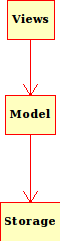
\includegraphics[width=1cm]{../design/grobentwurf.png}
    \end{center}
\end{frame}
\begin{frame}
    \frametitle{Feinentwurf}
    \begin{itemize}
        \item Verfeinerung des Views-Moduls
        \item Definition der Model-Eigenschaften
        \item Festlegung der Strukturen zum Datenaustausch
        \item Definition des Storage-Interfaces
    \end{itemize}
\end{frame}
\begin{frame}
    \frametitle{Feinentwurf}
    \begin{center}
        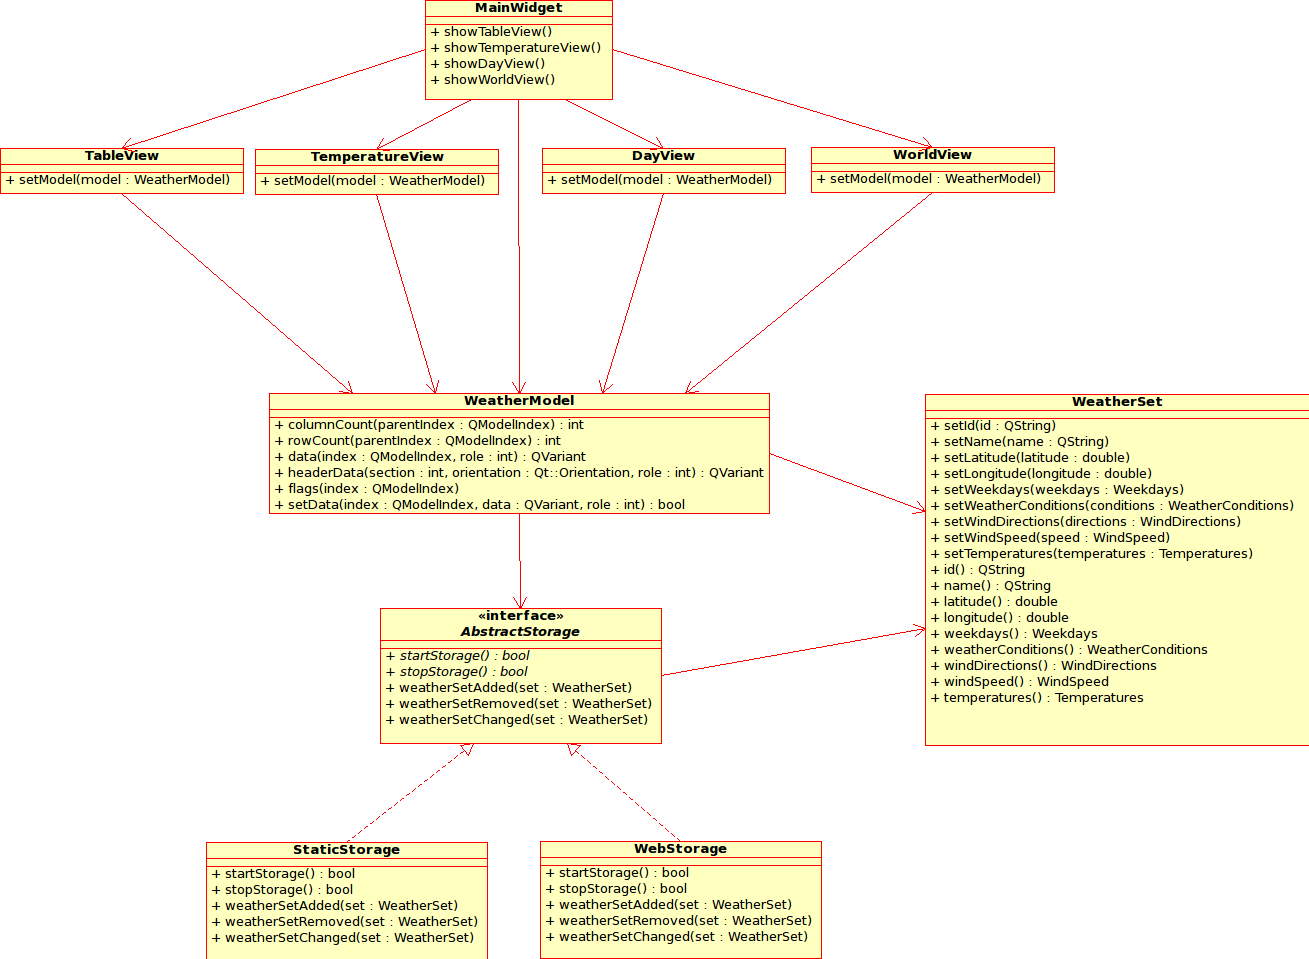
\includegraphics[width=10cm]{../design/feinentwurf.png}
    \end{center}
\end{frame}
\begin{frame}
    \frametitle{Allgemeines zur Entwicklung}
    \begin{itemize}
        \item Basiert auf C++/Qt
        \begin{itemize}
          \item Entwicklung unter Linux
          \item Produkt lauff\"ahig unter MS Windows
        \end{itemize}
        \item Nutzung des MVC-Frameworks von Qt
    \end{itemize}
\end{frame}

% \begin{frame}[fragile]
%     \frametitle{Beispiel: Proxy Model}
% \begin{tiny}
% \begin{verbatim}
% class LocationFilterProxy : public QSortFilterProxyModel
% {
%   Q_OBJECT
%   public:
%     LocationFilterProxy(QObject *parent)
%       : QSortFilterProxyModel(parent) {}
%
%   public Q_SLOTS:
%     void setLocationName(const QString &locationName)
%     {
%       mLocationName = locationName;
%       invalidateFilter();
%     }
%
%   protected:
%     virtual bool filterAcceptsRow(int row, const QModelIndex&) const
%     {
%       if (mLocationName.isEmpty())
%         return true;
%
%       const QModelIndex index = sourceModel()->index(row, 0);
%       const QString location = index.data(WeatherModel::NameRole).toString();
%
%       return location.toLower().contains(mLineEdit->text().toLower());
%     }
%
%   private:
%     QString *mLocationName;
% };
% \end{verbatim}
% \end{tiny}
% \end{frame}

\begin{frame}
    \frametitle{Demo}
    \begin{center}
        \large{Programmvorf\"uhrung}
    \end{center}
\end{frame}
